\chapter{評価手法と結果}
\label{chap:evaluation}
\section{本提案の評価概要と予想}
\ref{section:要件1}で述べた通り, リンク障害による配送遅延の増加の発生後, 
Contact Planの臨時更新を行うと, そのリンク情報がすべてのノードに伝搬し
再計算が行われる時間の間, 一時的にContact Planの不整合が発生する. 

\section{要件1に対するシミュレーション結果}
\label{section:要件1に対するシミュレーション結果}
本章では, \ref{chap:implementation_and_experimentation}で
述べたシミュレーションにおける結果についてまとめる. 
\ref{section:経路収束までの所要時間}では, 
\ref{section:要件1}で述べた経路収束までの所要時間についての
シミュレーション結果について, \ref{section:経路収束後の到達遅延}では
\ref{section:要件2}で述べた経路収束後の配送遅延についての
シミュレーション結果について述べる. 


\begin{table}[tbh]
    \centering
    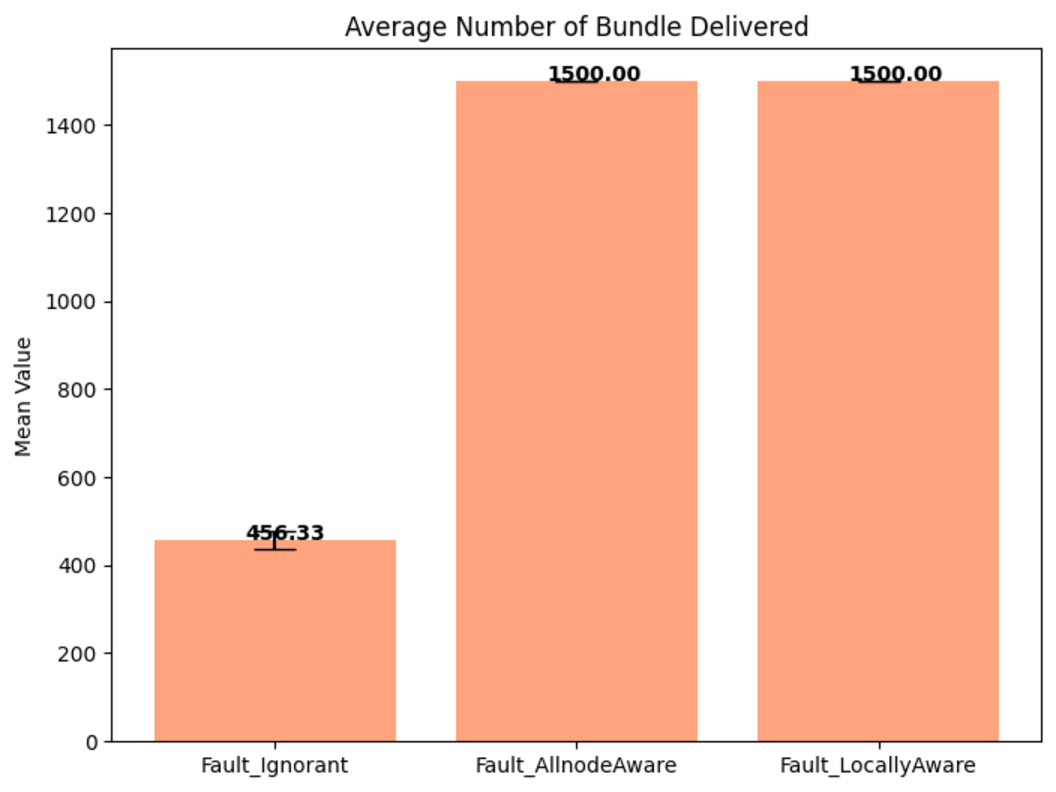
\includegraphics[width=0.7\textheight]{results/results_20250116/moon_bundle.pdf}
    \caption{バンドルの到達率}
    \label{fig:graph_bundle_earth_moon}
    \begin{minipage}{\textwidth}
        \centering
        \vspace{3mm}
        地球・月間シナリオにおけるノード6に向けたBundleの平均到達率
    \end{minipage}
\end{table}

\begin{table}[tbh]
    \centering
    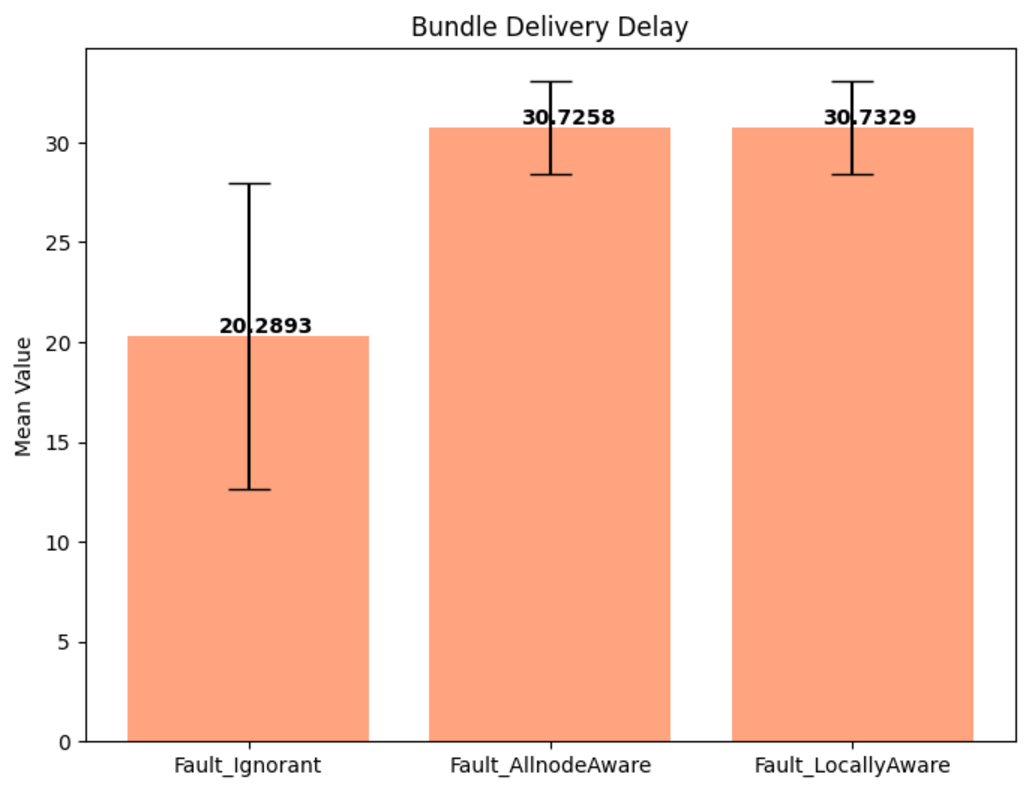
\includegraphics[width=0.7\textheight]{results/results_20250116/moon_delay.pdf}
    \caption{バンドルの到達遅延}
    \label{fig:graph_bundle_earth_moon}
    \begin{minipage}{\textwidth}
        \centering
        \vspace{3mm}
        地球・月間シナリオにおけるノード6に向けたBundleの到達遅延
    \end{minipage}
\end{table}

\subsection{経路収束までの所要時間}
\label{section:経路収束までの所要時間}
\ref{section:要件1}で述べた通り, リンク障害による配送遅延の増加の発生後, 
Contact Planの臨時更新を行うと, そのリンク情報がすべてのノードに伝搬し
再計算が行われる時間の間, 一時的にContact Planの不整合が発生し, 経路収束までの所要時間の
間は遅延が大きくなることが予想される. 
\begin{figure}[tbh]
    \centering
    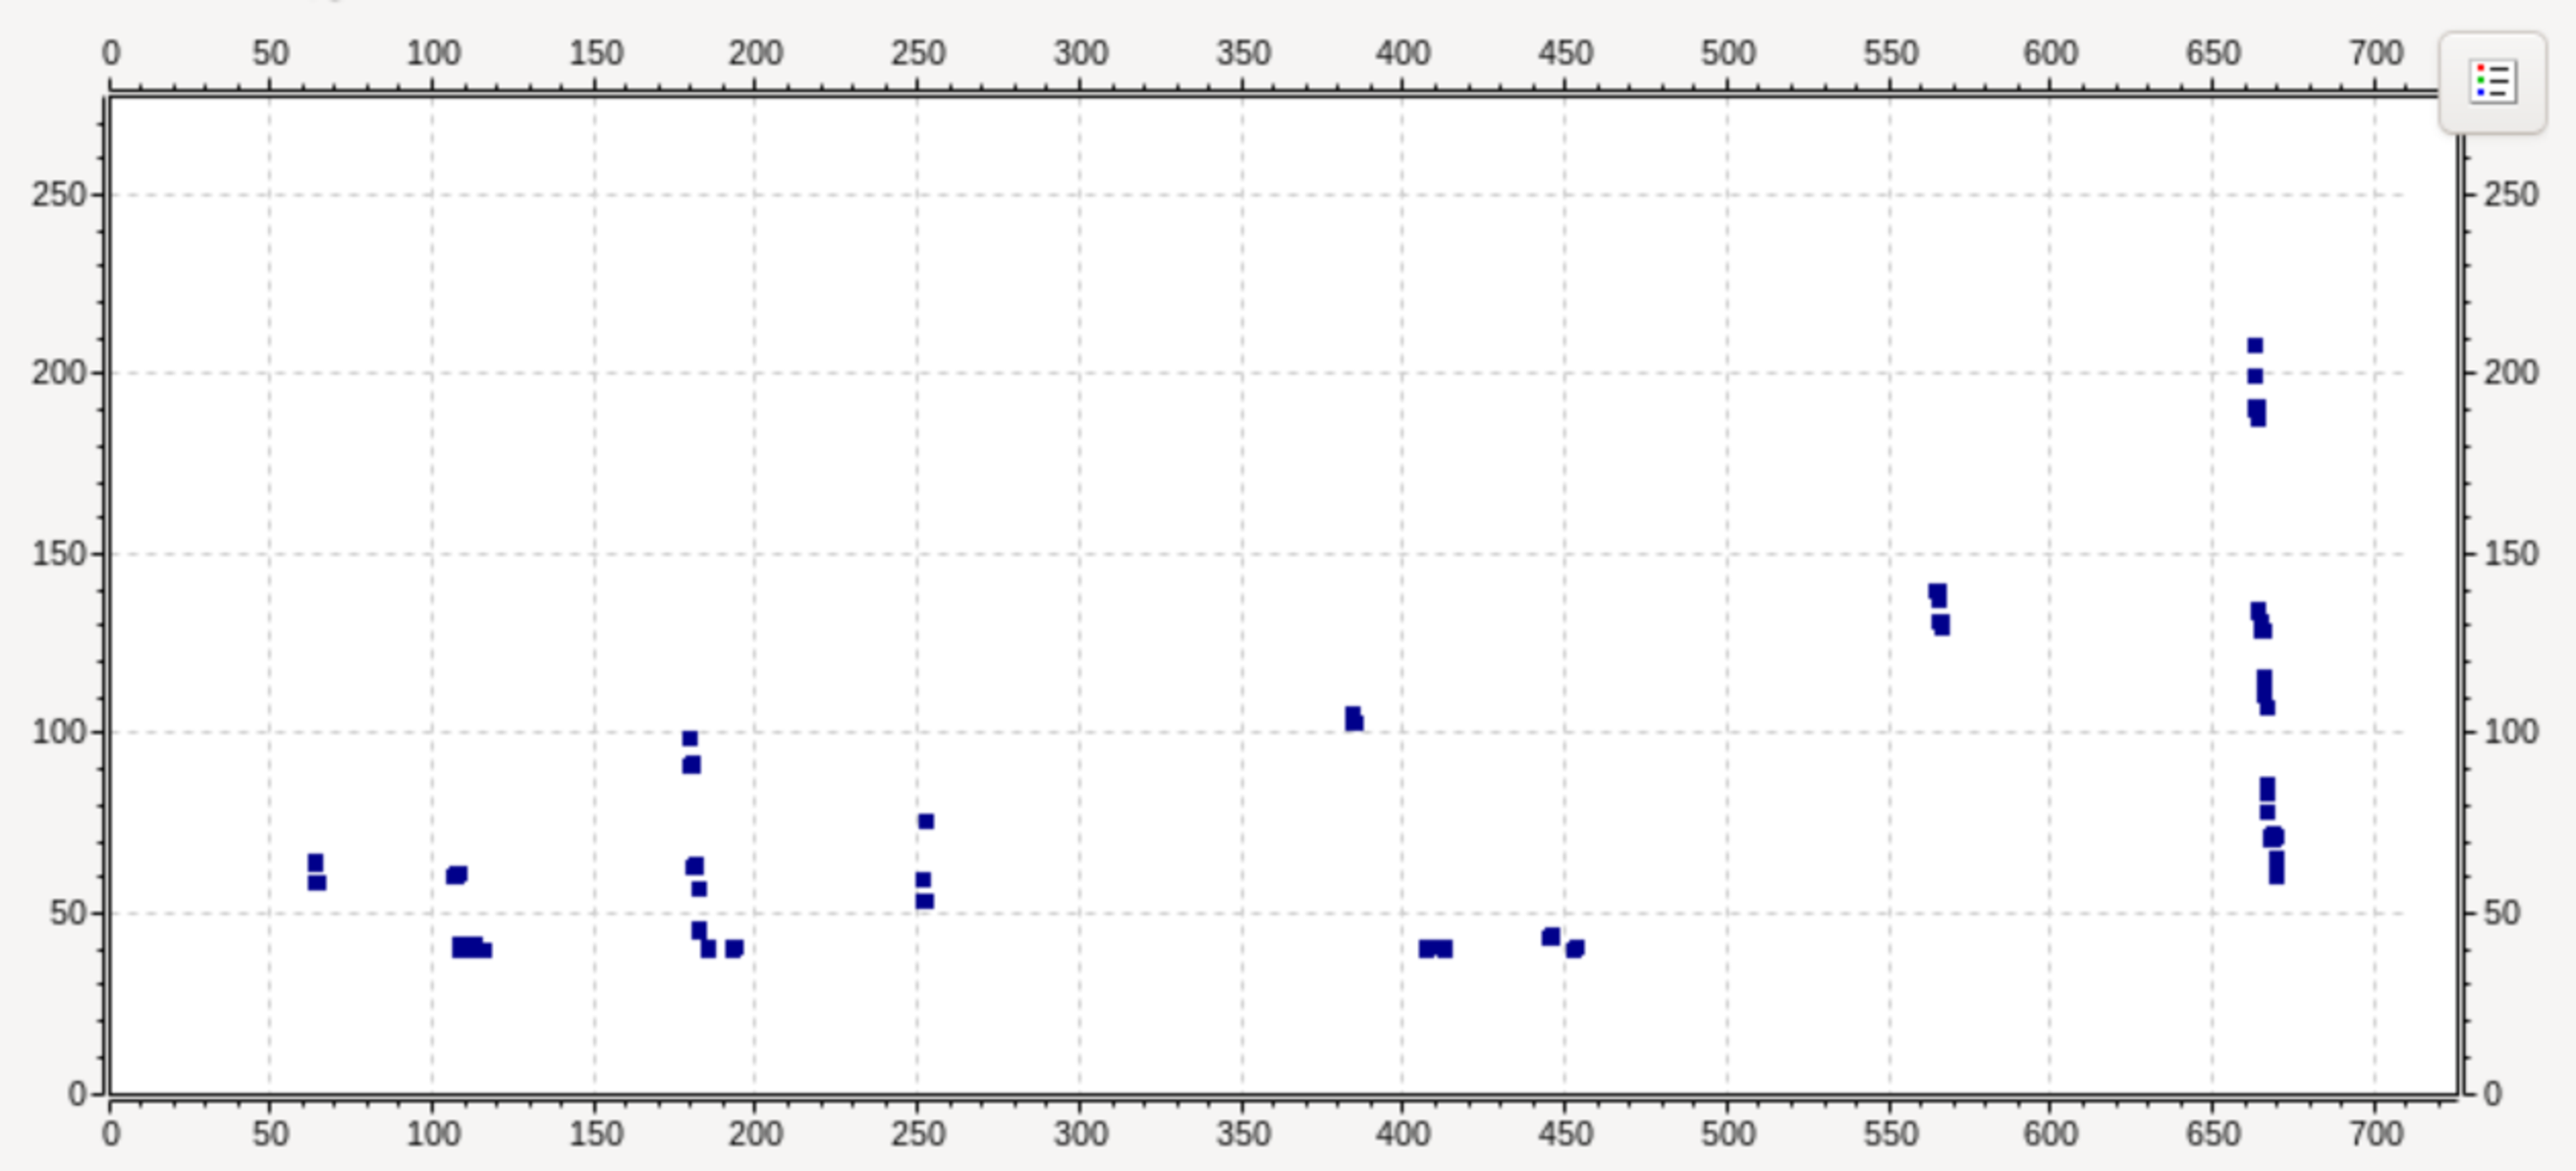
\includegraphics[width=0.7\textheight]{img/thesis_sample_delay_time.pdf}
    \caption{ノード6に向けたBundleの到達遅延の時間変化(地球・月間のシミュレーション)}
    \label{fig:delay_time_variation_earth_moon}
    \begin{minipage}{\textwidth}
        \raggedright
        \vspace{3mm}
        ノード6における, シミュレーション内での全到達Bundleの到達遅延の最大値・平均値・最小値. 
        本シミュレーションにおいては, \ref{section:シミュレーションで用いるバンドルトラフィック}
        で述べたように, ノード6に対するBundleトラフィックのみを生成しているため, 
        ノード6のみの到達遅延を示す. 
    \end{minipage}
\end{figure}

\begin{figure}[tbh]
    \centering
    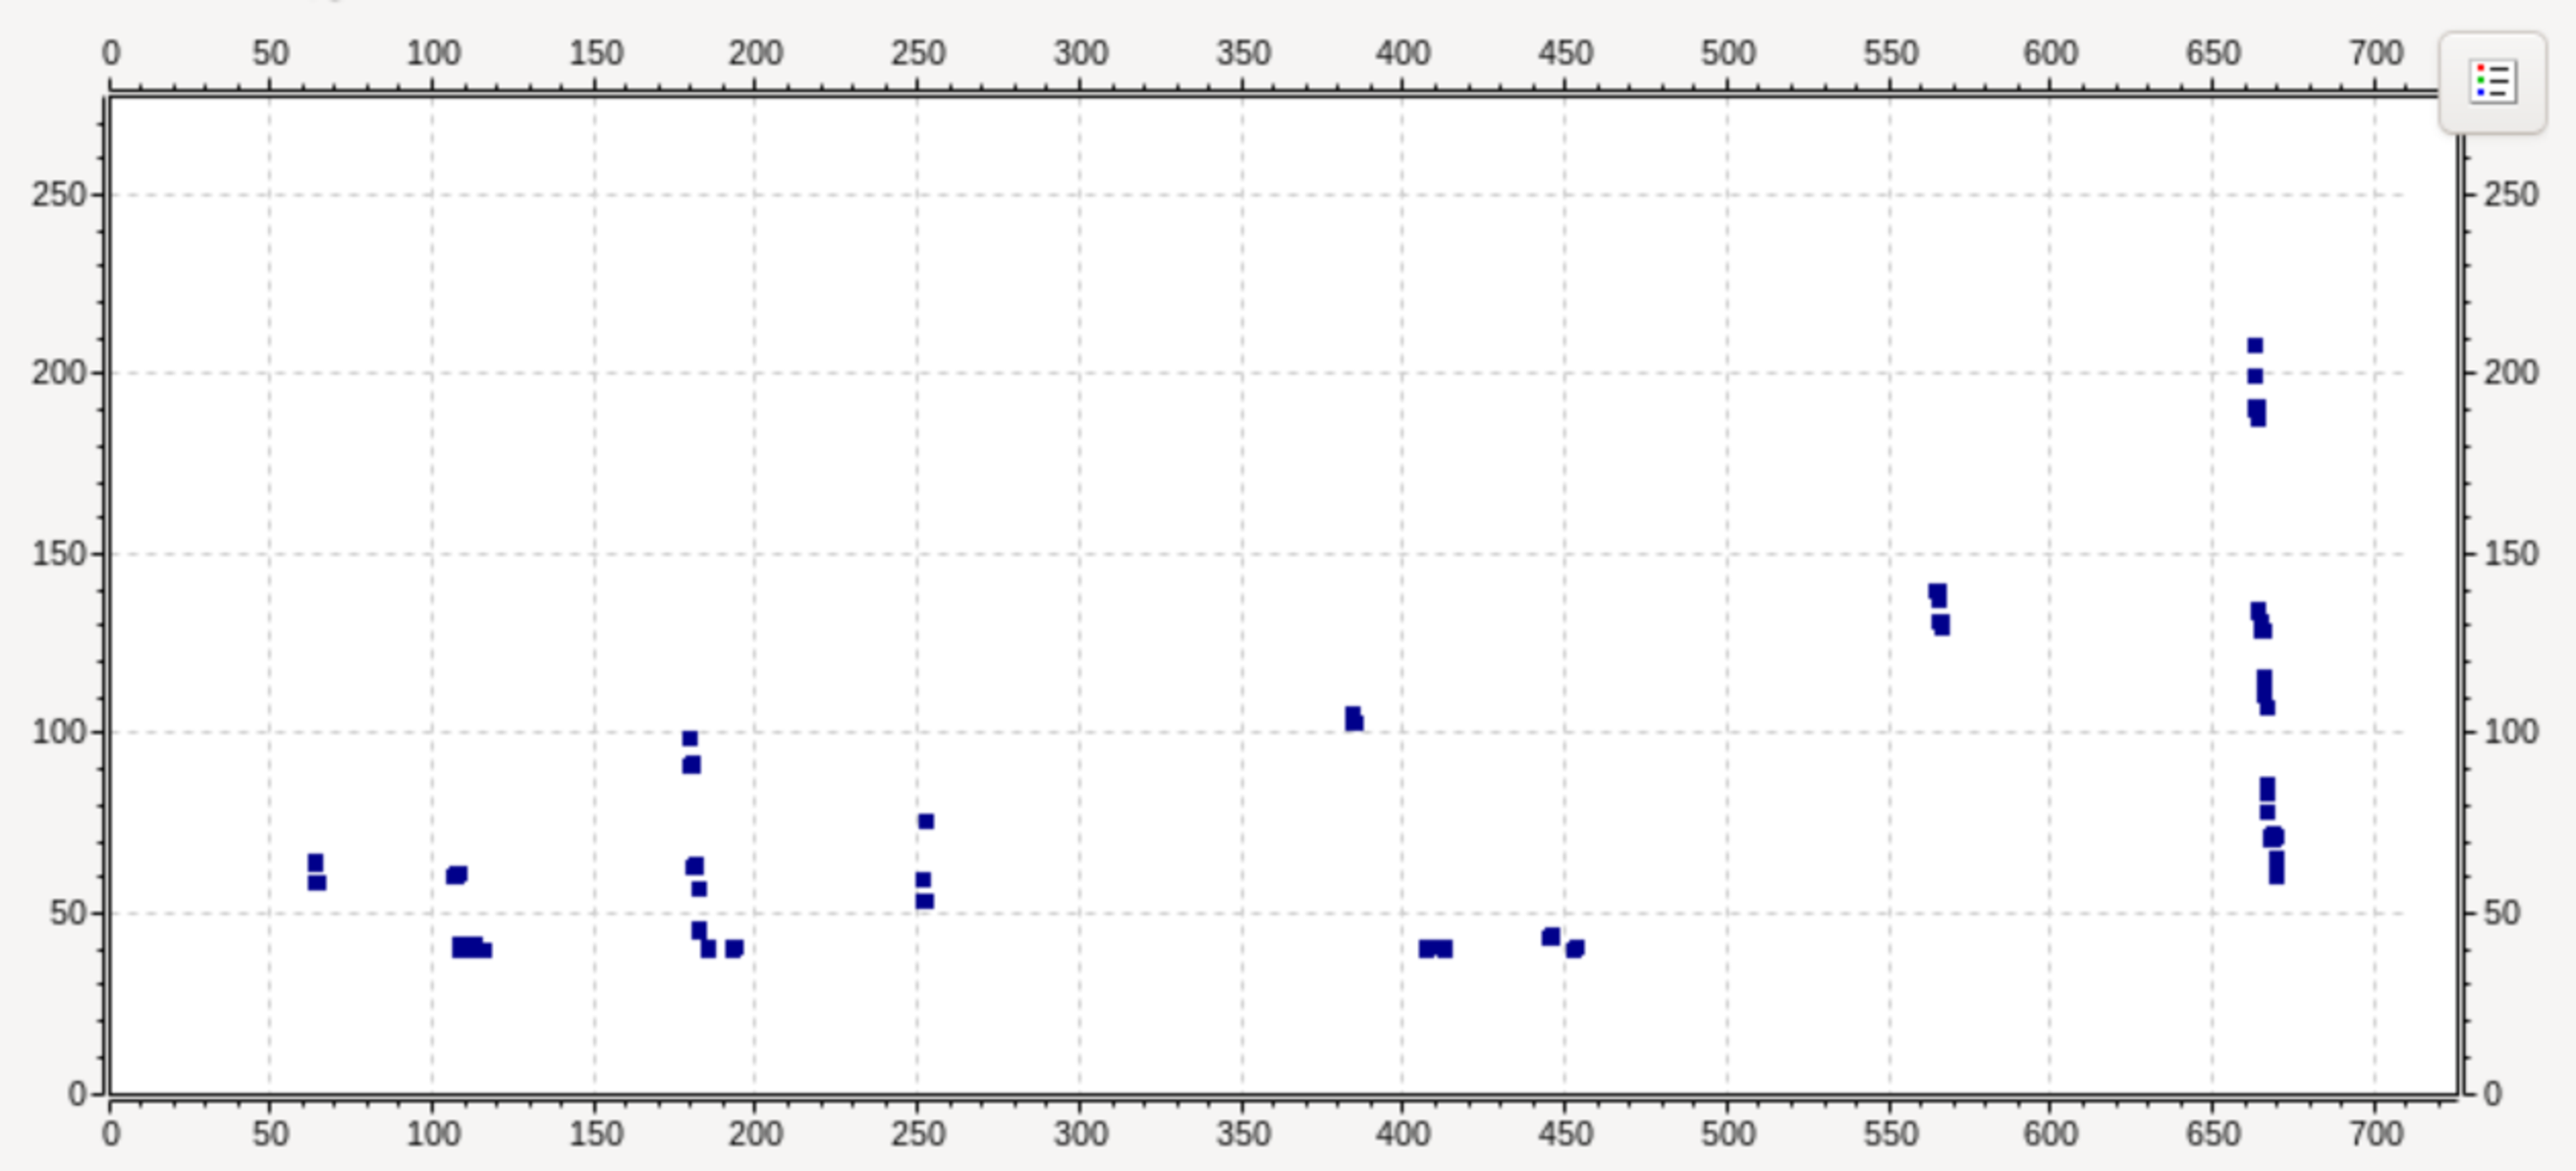
\includegraphics[width=0.7\textheight]{img/thesis_sample_delay_time.pdf}
    \caption{ノード6に向けたBundleの到達遅延の時間変化(地球・火星間のシミュレーション)}
    \label{fig:delay_time_variation_earth_mars}
    \begin{minipage}{\textwidth}
        \raggedright
    \end{minipage}
\end{figure}

\begin{figure}[tbh]
    \centering
    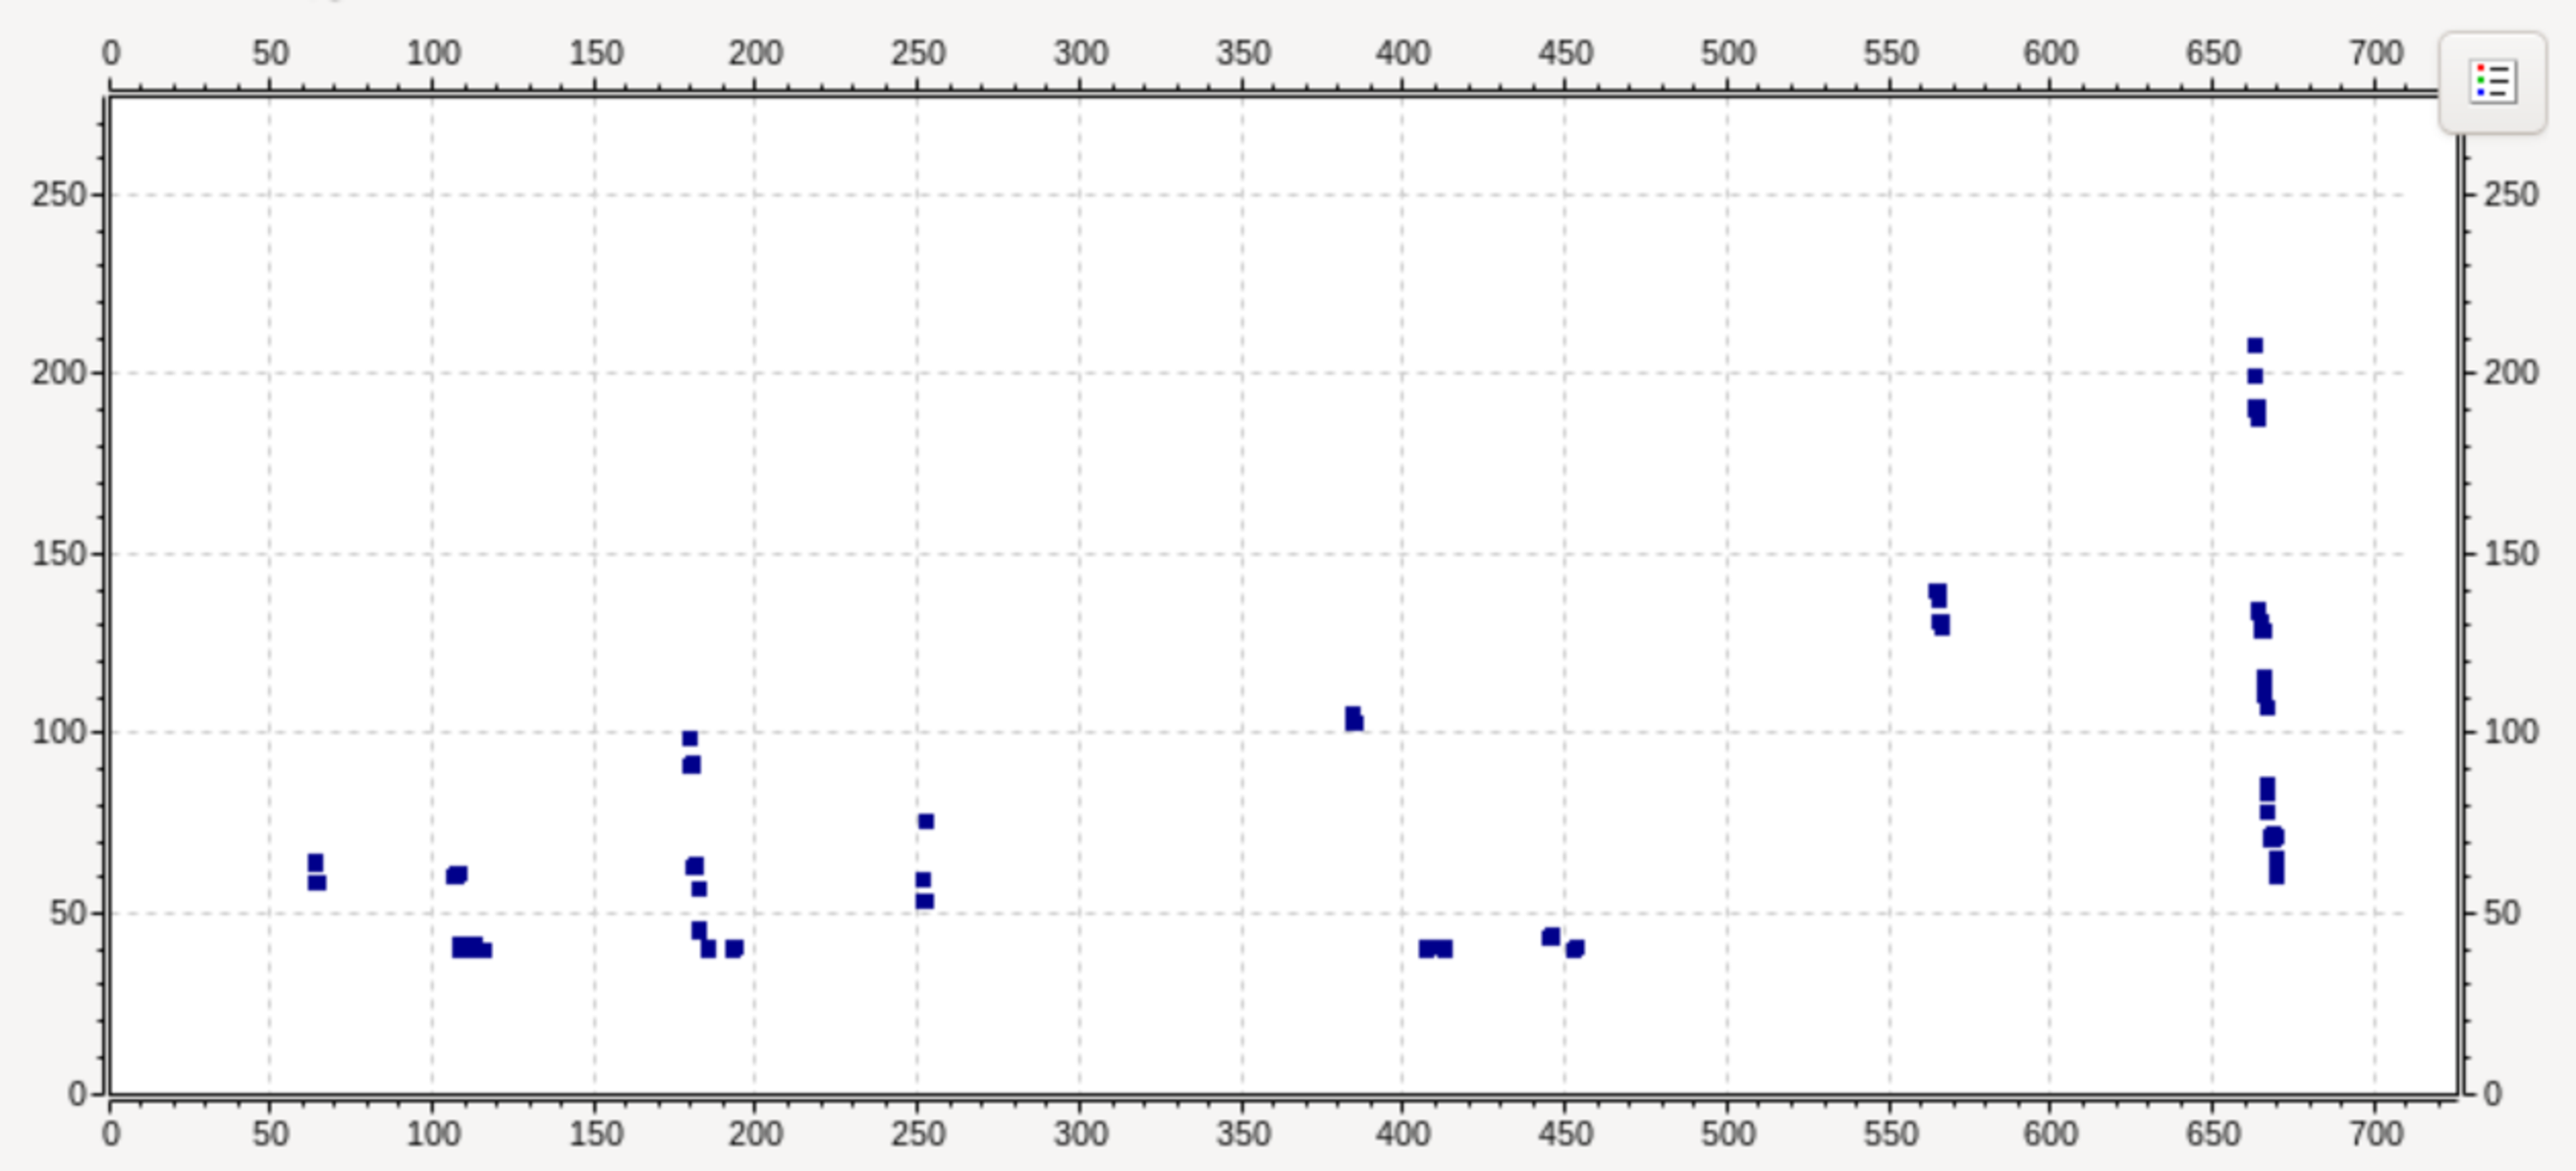
\includegraphics[width=0.7\textheight]{img/thesis_sample_delay_time.pdf}
    \caption{ノード6に向けたBundleの到達遅延の時間変化(火星・火星の衛星間のシミュレーション)}
    \label{fig:delay_time_variation_mars_marssat}
    \begin{minipage}{\textwidth}
        \raggedright
    \end{minipage}
\end{figure}

\subsection{経路収束後の到達遅延}
\label{section:経路収束後の到達遅延}
\ref{section:要件2}で述べた通り, リンク障害による配送遅延の増加の発生後, 
Contact Planの臨時更新を行うと, そのリンク情報がすべてのノードに伝搬し
再計算が行われる時間, すなわち収束までの時間

